\documentclass[5pt]{article}
\usepackage{mathptmx,amsmath}
\usepackage{pdfslide2,pause}
\usepackage{eurosym}
\usepackage[portuguese,english]{babel}
\usepackage{kerkis}
\usepackage{colortbl} % used to highlight row or columns of tables. http://www.tug.org/pracjourn/2007-1/mori/mori.pdf
\usepackage[small]{caption} % more option on http://www.dd.chalmers.se/latex/Docs/PDF/caption.pdf
\usepackage[tight,scriptsize]{subfigure}
\usepackage{lastpage}
\usepackage{chngcntr}
\usepackage[absolute,overlay]{textpos}
\usepackage{tabto}
\usepackage{animate}
%\usepackage{listings}
\captionsetup{labelformat=empty,skip=-0.8cm}

%\lstset{
%    language=Matlab,                % choose the language of the code
%    basicstyle=\ttfamily\tiny,       % the size of the fonts that are used for the code
%    numbers=none,                   % where to put the line-numbers
%    numberstyle=\tiny,              % the size of the fonts that are used for the line-numbers
%    stepnumber=1,                   % the step between two line-numbers. If it's 1 each line will be numbered
%    numbersep=5pt,                  % how far the line-numbers are from the code
%    backgroundcolor=\color{white},  % choose the background color. You must add \usepackage{color}
%    showspaces=false,               % show spaces adding particular underscores
%    showstringspaces=false,         % underline spaces within strings
%    showtabs=false,                 % show tabs within strings adding particular underscores
%    tab=\rightarrowfill,
%    frame=none,	                    % adds a frame around the code
%    tabsize=2,	                    % sets default tabsize to 2 spaces
%    captionpos=b,                   % sets the caption-position to bottom
%    breaklines=true,                % sets automatic line breaking
%    breakatwhitespace=false,        % sets if automatic breaks should only happen at whitespace
%    title=\lstname,                 % show the filename of files included with \lstinputlisting; also try caption instead of title
%    escapeinside={\%*}{*)},          % if you want to add a comment within your code
%    morekeywords={ifftshift,fftshift},
%    keywordstyle=\bfseries\color[rgb]{0,0,0.3},
%    commentstyle=\color[rgb]{0.133,0.5,0.133}
%}
%\lstset{
%    emph={function,end,for,if,while},
%    emphstyle=\bfseries\color[rgb]{0.6,0,0},
%}

\definecolor{itblue}{rgb}{0.0,0.0,0.5}
\definecolor{itred}{rgb}{0.82,0.18,0.24}
\newcommand{\pageNum}{
    \begin{picture}(0,0)(0,0)
        \put(-15,-390){
            \begin{minipage}{1.8cm}
            \end{minipage}
        }
    \end{picture}
}
\newcommand{\cb}[1]{{\color{itblue} #1}}%
\newcommand{\cred}[1]{{\color{itred} #1}}%
\newcommand{\bb}[1]{{\textbf{\color{itblue} #1}}}%
\newcommand{\br}[1]{{\textbf{\color{itred} #1}}}%
\renewcommand{\labelitemi}{\textcolor{itred}{\normalsize $\bullet$}}
\renewcommand{\labelitemii}{\textcolor{itblue}{$\bullet$}}
\newcommand{\mysection}[1]{\section*{\pageNum\color{itred}\sffamily #1}\vspace*{0.5cm}\overlay{it_1.png}\sffamily}%
\newcommand{\ITfootnote}[1]{\hspace{1.8cm}\begin{minipage}{13cm}\tiny{#1}\end{minipage}}
\newcommand{\edfaGain}{$G=\exp\left(\frac{\alpha}{2}L_{span}\right)$}
\newenvironment{reference}{
    \begin{textblock*}{0.7\textwidth}(32mm,137mm)\tiny\noindent\bgroup\color{black}
}
{
    \egroup\end{textblock*}
}


\graphicspath{{./Figures/}}
\pagestyle{title}

\hyphenpenalty=50000
\tolerance=10000

\setlength{\textheight}{1.5\textheight}

%%%%%%%%%%%%%%%%%%%%%%%%%%%%%%%%%%%%%%%%%%%%%%%%%%%%%%%%%%%%%%%%%%%%%%%%%%%%%%%%%%%%%%%%%%%%%%%%%%%
%%%%%%%%%%%%%%%%%%%%%%%%%%%%%%%%%%%%%%%%%%%%%%%%%%%%%%%%%%%%%%%%%%%%%%%%%%%%%%%%%%%%%%%%%%%%%%%%%%%

\begin{document}

%************************************************************************************************
%                                          SLIDE
%************************************************************************************************
\pagenumbering{roman}
\begin{titlepage}  \overlay{it_0.png}

\color{itblue} \sffamily \noindent \small
\hspace*{1cm}  Universidade de Aveiro\\ %Instituto\\ Superior T�cnico, Instituto de Telecomunica��es\\
\hspace*{1cm}  2017-2018\\ %Lisboa, 14th of February, 2013\\

\vspace*{1cm}
\begin{center}
    \color{black} \sffamily \noindent \Large
    \br{Simplified Coherent Transceivers for Optical Communication Networks\\}
\end{center}
\vspace{6mm}
\begin{center}
    \color{black}
    \textbf{Romil Patel\\}
    {(romilkumar@ua.pt)}
\end{center}

\vspace{0.0mm}
\scriptsize
\begin{center}
Department of Electronics, Telecommunications and Informatics,\\
University of Aveiro, Aveiro, Portugal\\
Instituto de Telecomunica\c{c}\~{o}es, Aveiro, Portugal\\
\end{center}

\vspace{1.0cm}
\hspace*{13.2cm}\tiny \copyright 2005, it - instituto de telecomunica\c{c}\~{o}es\hfill

\end{titlepage}


\renewcommand{\headsep}{-25pt}
\pagenumbering{arabic}



%--------------------------------------------------------------------------------------------------
%------------ SLIDE-------
\mysection{Kramers-Kronig transceiver}\large
\vspace{0cm}

The Kramers-Kronig relations are bidirectional mathematical relations, connecting the real and imaginary parts of any complex function that is analytic in the upper half-plane. For instance, a signal $x(t)=x_r(t) + i x_i(t)$ satisfies the Kramers-Kronig relationship if,
\begin{equation*}
\begin{split}
x_{r}(t) &=-\frac{1}{\pi} p.v. \int_{-\infty}^{\infty} \frac{x_{i}(t')}{t-t'} dt' \\ \\
x_{i}(t) &=\frac{1}{\pi} p.v. \int_{-\infty}^{\infty} \frac{x_{r}(t')}{t-t'} dt' \\
\end{split}
\label{KK}
\end{equation*}
This relationship imposes that the real and the imaginary parts of the signal are related to each other though Hilbert transform. Therefore, if we have the real part of the signal then the imaginary part can be calculated by its Hilbert transform.


%--------------------------------------------------------------------------------------------------
%------------ SLIDE -------------------------------------------------------------------------------

\mysection{ \\[-5mm]1. What is Hilbert transform?}\large
\vspace*{0mm}
If we consider a filter $H(\omega)$ that has a unity magnitude response for all frequencies and the phase response is $-\pi/2$ for all positive frequencies and $\pi/2$ for negative frequencies.
\begin{figure}[hbt]
	\centering
	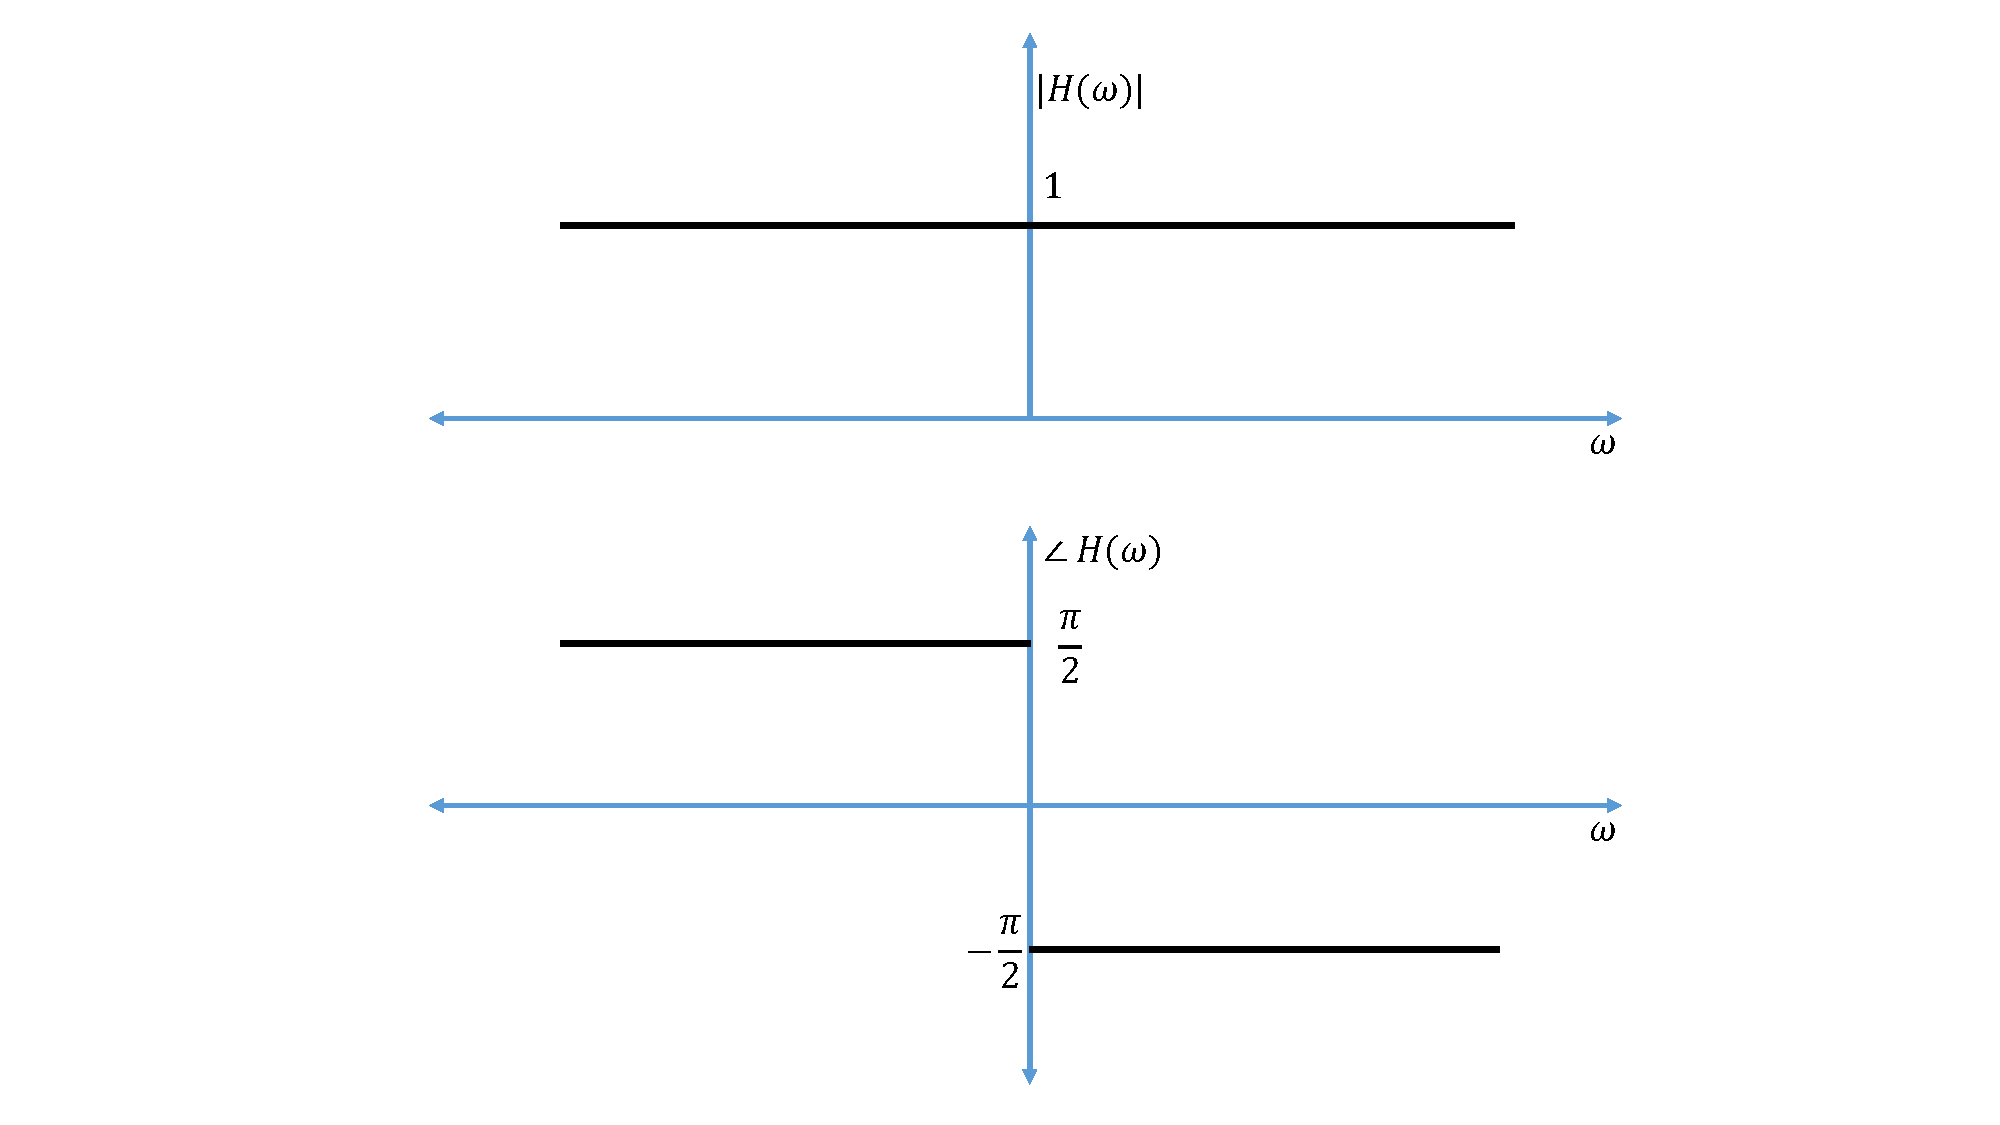
\includegraphics[width=0.75\textwidth, height=6cm]{./figures/HT.pdf}
    \vspace{10mm}
    \caption{Magnitude and phase of Hilbert transform filter}\label{Hilbert_Transformer}
\end{figure}

%--------------------------------------------------------------------------------------------------
%------------ SLIDE--------------------------------------------------------------------------------
\mysection{}
The transfer function of this filter is given by
\begin{equation}
\begin{split}
H(\omega)=-isgn(\omega)
\end{split}
\label{}
\end{equation}

The inpulse response of this filter can be given as,
\begin{equation}
\begin{split}
h(t)&=\frac{1}{\pi t}
\end{split}
\label{}
\end{equation}

When this filter driven by an arbitrary signal $s(t)$, the filter produces the output as,
\begin{equation}
\begin{split}
\hat{s}(t)&=s(t) * h(t) = \int_{-\infty}^{\infty} \dfrac{s(u)}{\pi(t-u)}du\\
\end{split}
\label{}
\end{equation}
The function $\hat{s}(t)$ is called the Hilbert transform if $s(t)$. Note that
\begin{equation}
\begin{split}
\mathcal{F}[\hat{s}(t)]=H(\omega)S(\omega)=-isgn(\omega)S(\omega)
\end{split}
\label{}
\end{equation}

%--------------------------------------------------------------------------------------------------
%------------ SLIDE--------------------------------------------------------------------------------
\mysection{2. What is the SSB signal and how it can be generated?}\large
\vspace{0cm}
By definition, the SSB is the signal which contains either upper sideband or lower sideband and hence it reduces the spectral occupancy by half. In another words, SSB signal is the frequency translated version of an analytical signal.\\
\begin{itemize}
\item \textbf{Analytical Signal}  : An analytic signal is a complex-valued signal that has no negative frequency components, and its real and imaginary parts are related to each other by the Hilbert transform.
\begin{equation}
s_a(t)=s(t)+i\hat{s}(t)
\label{Analytical signal}
\end{equation}
\end{itemize}
where, $s_a(t)$ is an analytical signal and $\hat{s}(t)$ is the Hilbert transform of the signal ${s}(t)$. Such analytical signal can be used to generate Single Sideband Signal (SSB) signal.

%--------------------------------------------------------------------------------------------------
%------------ SLIDE--------------------------------------------------------------------------------
\mysection{}\large
Since a SSB signal is the frequency translated version of an analytical signal, it can be generated as,
\begin{equation}
\begin{split}
{s}_{ssb}(t)&=Re\{s_a(t)  e^{i2\pi f_0 t}\}\\
&=Re\{[s(t)+i\hat{s}(t)] [cos(2\pi f_0t)+isin(2\pi f_0t)]\}\\
&=s(t)cos(2\pi f_0t)-\hat{s}(t)sin(2\pi f_0t)
\end{split}
\label{USB_SSB}
\end{equation}


%--------------------------------------------------------------------------------------------------
%------------ SLIDE-------
\mysection{3. What is minimum phase signal?}\large
\begin{itemize}
  \item A necessary and sufficient condition for a complex signal $A(t)$ to be minimum phase is that the curve described in a complex plane by $A(t)$ when $t\rightarrow -\infty$ to $t\rightarrow \infty$ \textbf{does not encircle the origin}.
  \item A minimum-phase signal has an useful property that the natural logarithm of the magnitude of the frequency response is related to the phase angle of the frequency response by the Hilbert transform.
\end{itemize}
\begin{figure}[hbt]
	\centering
	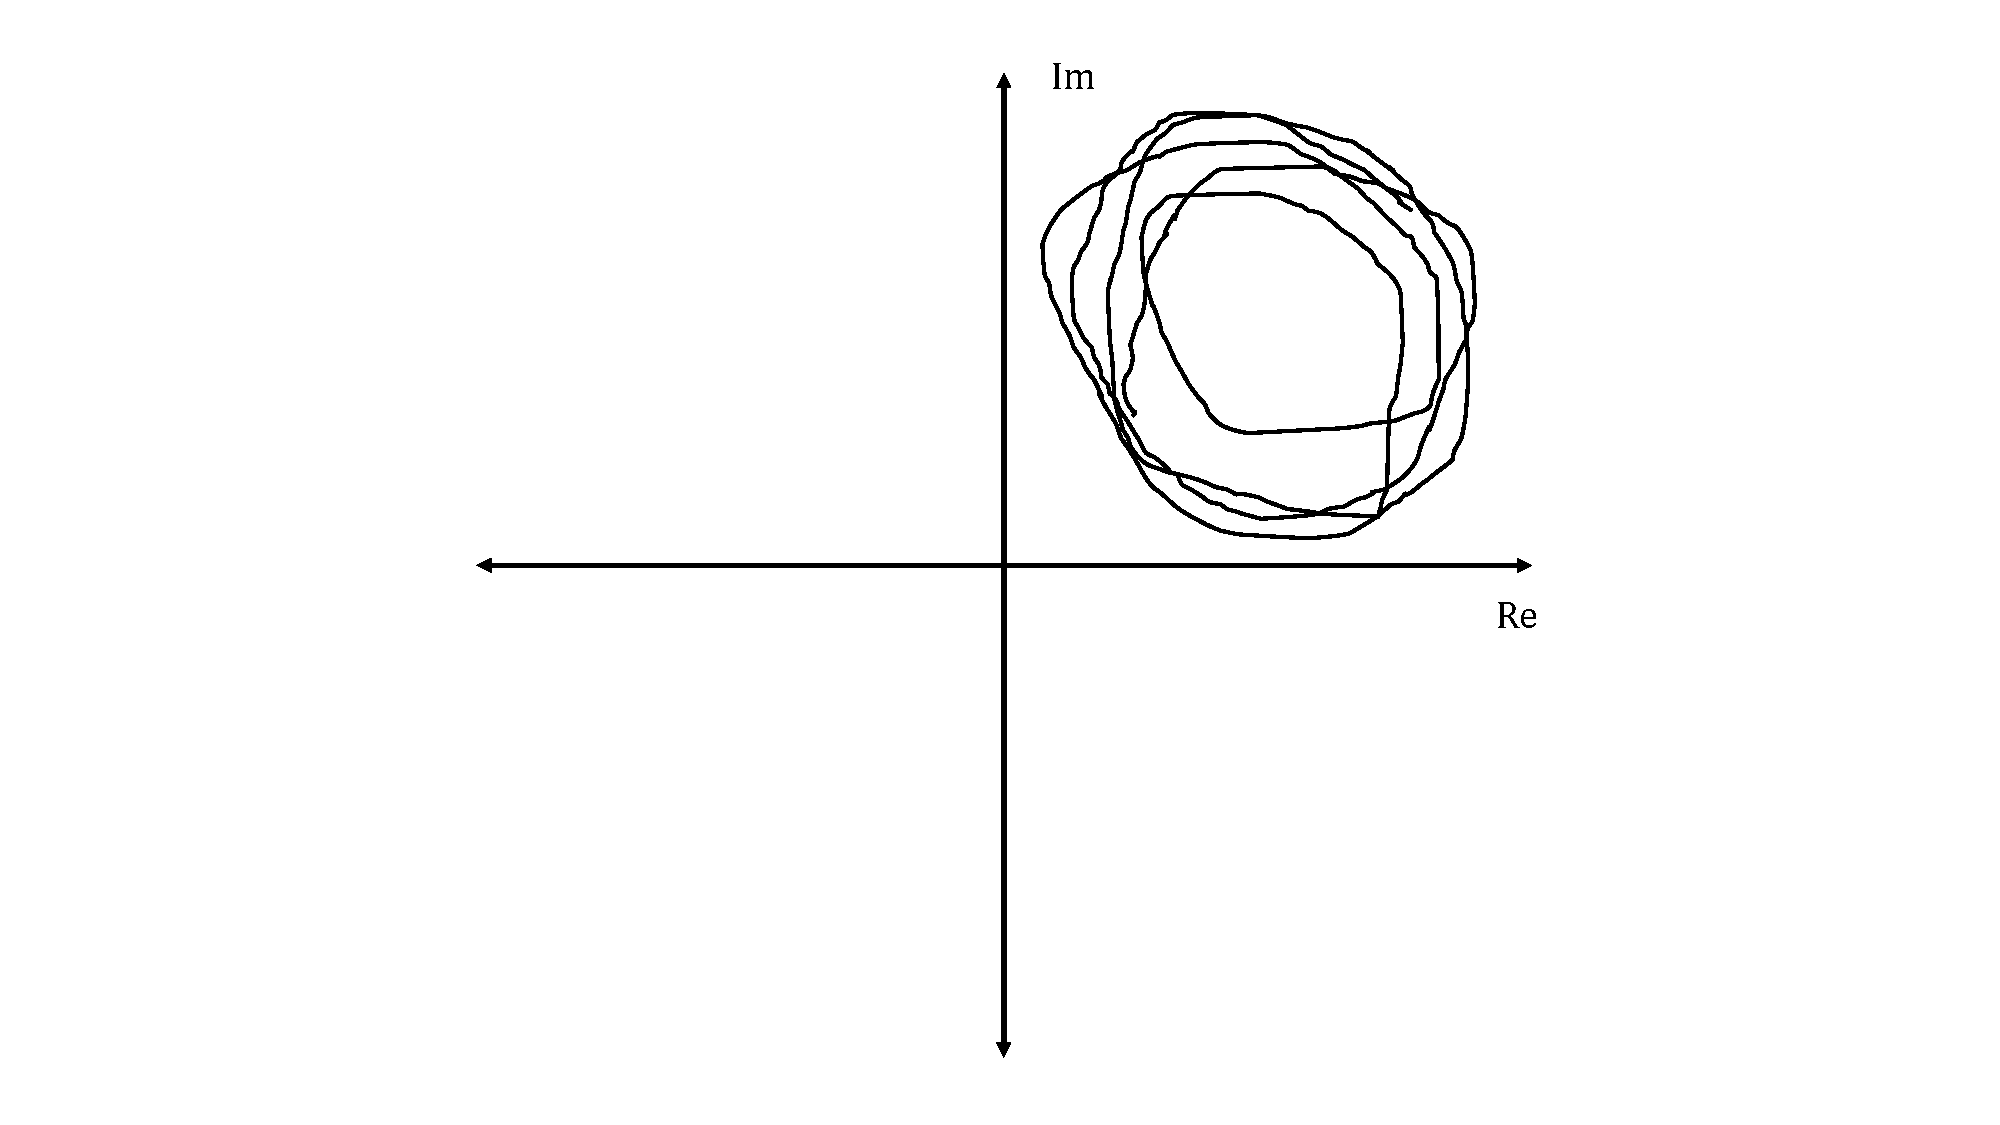
\includegraphics[width=0.5\textwidth, height=5cm]{./figures/MP_Signal.pdf}
    \vspace{5mm}
    \caption{Minumum Phase Signal}\label{}
\end{figure}

%--------------------------------------------------------------------------------------------------
%------------ SLIDE-------
\mysection{4. How we can use these signals and profit from them?}\large
\begin{itemize}
  \item \textbf{Analytical Signal:}\\
         If we denote an analytic signal $A_s(t)$ as,
        \begin{equation}
        A_s(t)=A_{s,r}(t)+iA_{s,i}(t)
        \label{Eq:5.31}
        \end{equation}
        then in the equation \ref{Eq:5.31}, the real and imaginary parts $A_{s,r}(t)$ and $A_{s,i}(t)$ are related through the Kramers-Kronig relation with each other as,
\begin{equation}
\begin{split}
A_{s,r}(t) &=-\frac{1}{\pi} p.v. \int_{-\infty}^{\infty} \frac{A_{s,i}(t')}{t-t'} dt' \\
A_{s,i}(t) &=\frac{1}{\pi} p.v. \int_{-\infty}^{\infty} \frac{A_{s,r}(t')}{t-t'} dt' \\
\end{split}
\label{Eq:5.38}
\end{equation}

\end{itemize}


%--------------------------------------------------------------------------------------------------
%------------ SLIDE-------
\mysection{}\large
\vspace{0cm}
\begin{itemize}
\item \textbf{Minimum Phase signal:}\\
    Given function $A(t)=A_{s}(t)+\bar{E}$ never encircles the origin for $t\in(-\infty,\infty)$.
\begin{equation}
G(t)=log\bigg[\dfrac{A(t)}{\bar{A}}\bigg]\\
\label{Eq:A1}
\end{equation}

Under the hypothesis of signal being minimum phase, the phase information can be reconstructed by from its intensity as,
\begin{equation}.
\begin{split}
\phi(t) &= \bar{\phi} + \frac{1}{2\pi} p.v. \int_{-\infty}^{\infty} \frac{log|A(t)|^2}{t-t'} dt'\\
\end{split}
\label{Eq:E1}
\end{equation}


\end{itemize}

%--------------------------------------------------------------------------------------------------
%------------ SLIDE-------
\mysection{Simulation setup}\large
\begin{itemize}
  \item \textbf{Transmitter setup}
  \begin{figure}[hbt]
	\centering
	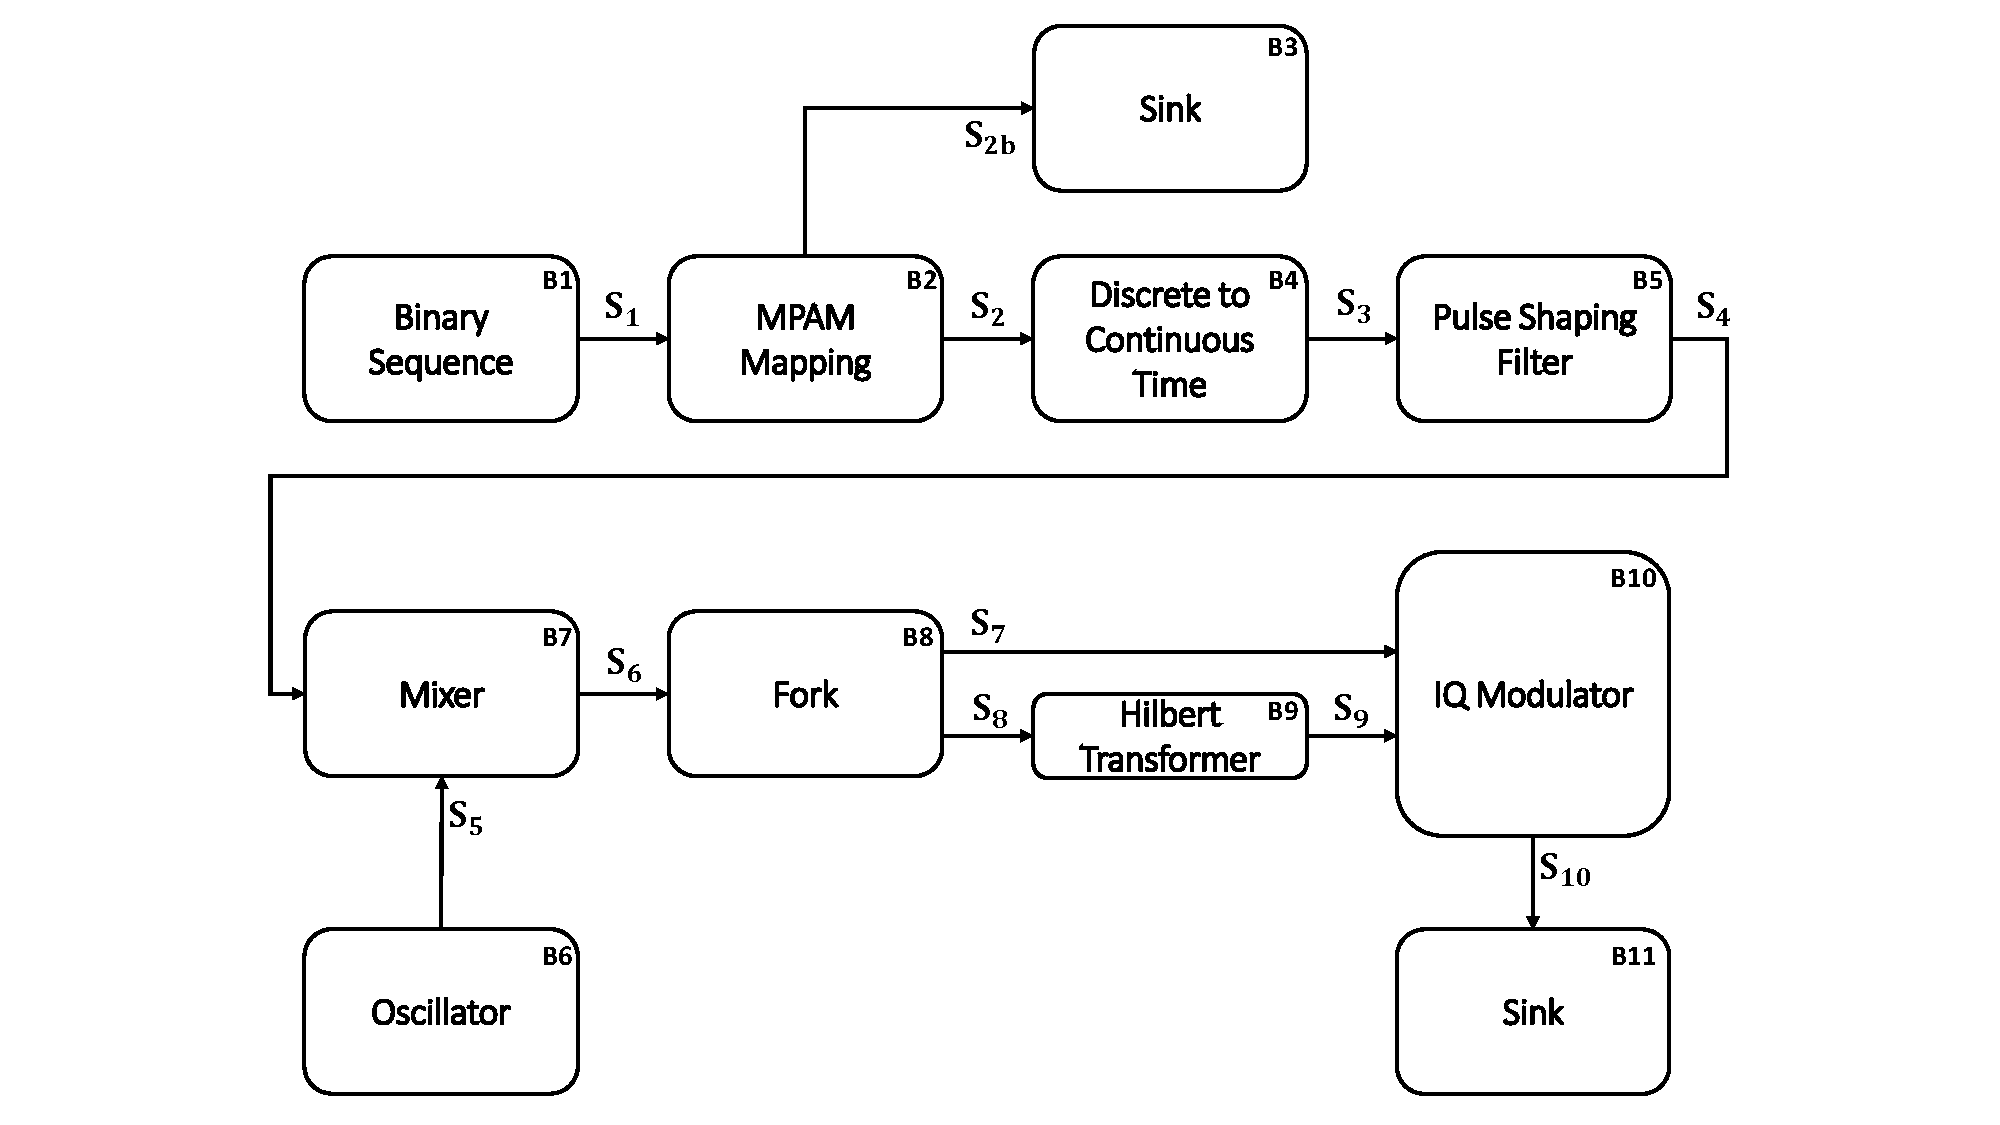
\includegraphics[width=1.0\textwidth, height=10cm]{./figures/Simulation_setup_Tx.pdf}
    \vspace{3mm}
    \caption{Transmitter simulation setup}\label{}
\end{figure}
\end{itemize}


%--------------------------------------------------------------------------------------------------
%------------ SLIDE-------
\mysection{Simulation setup}\large
\begin{itemize}
  \item \textbf{Receiver setup}
  \begin{figure}[hbt]
	\centering
	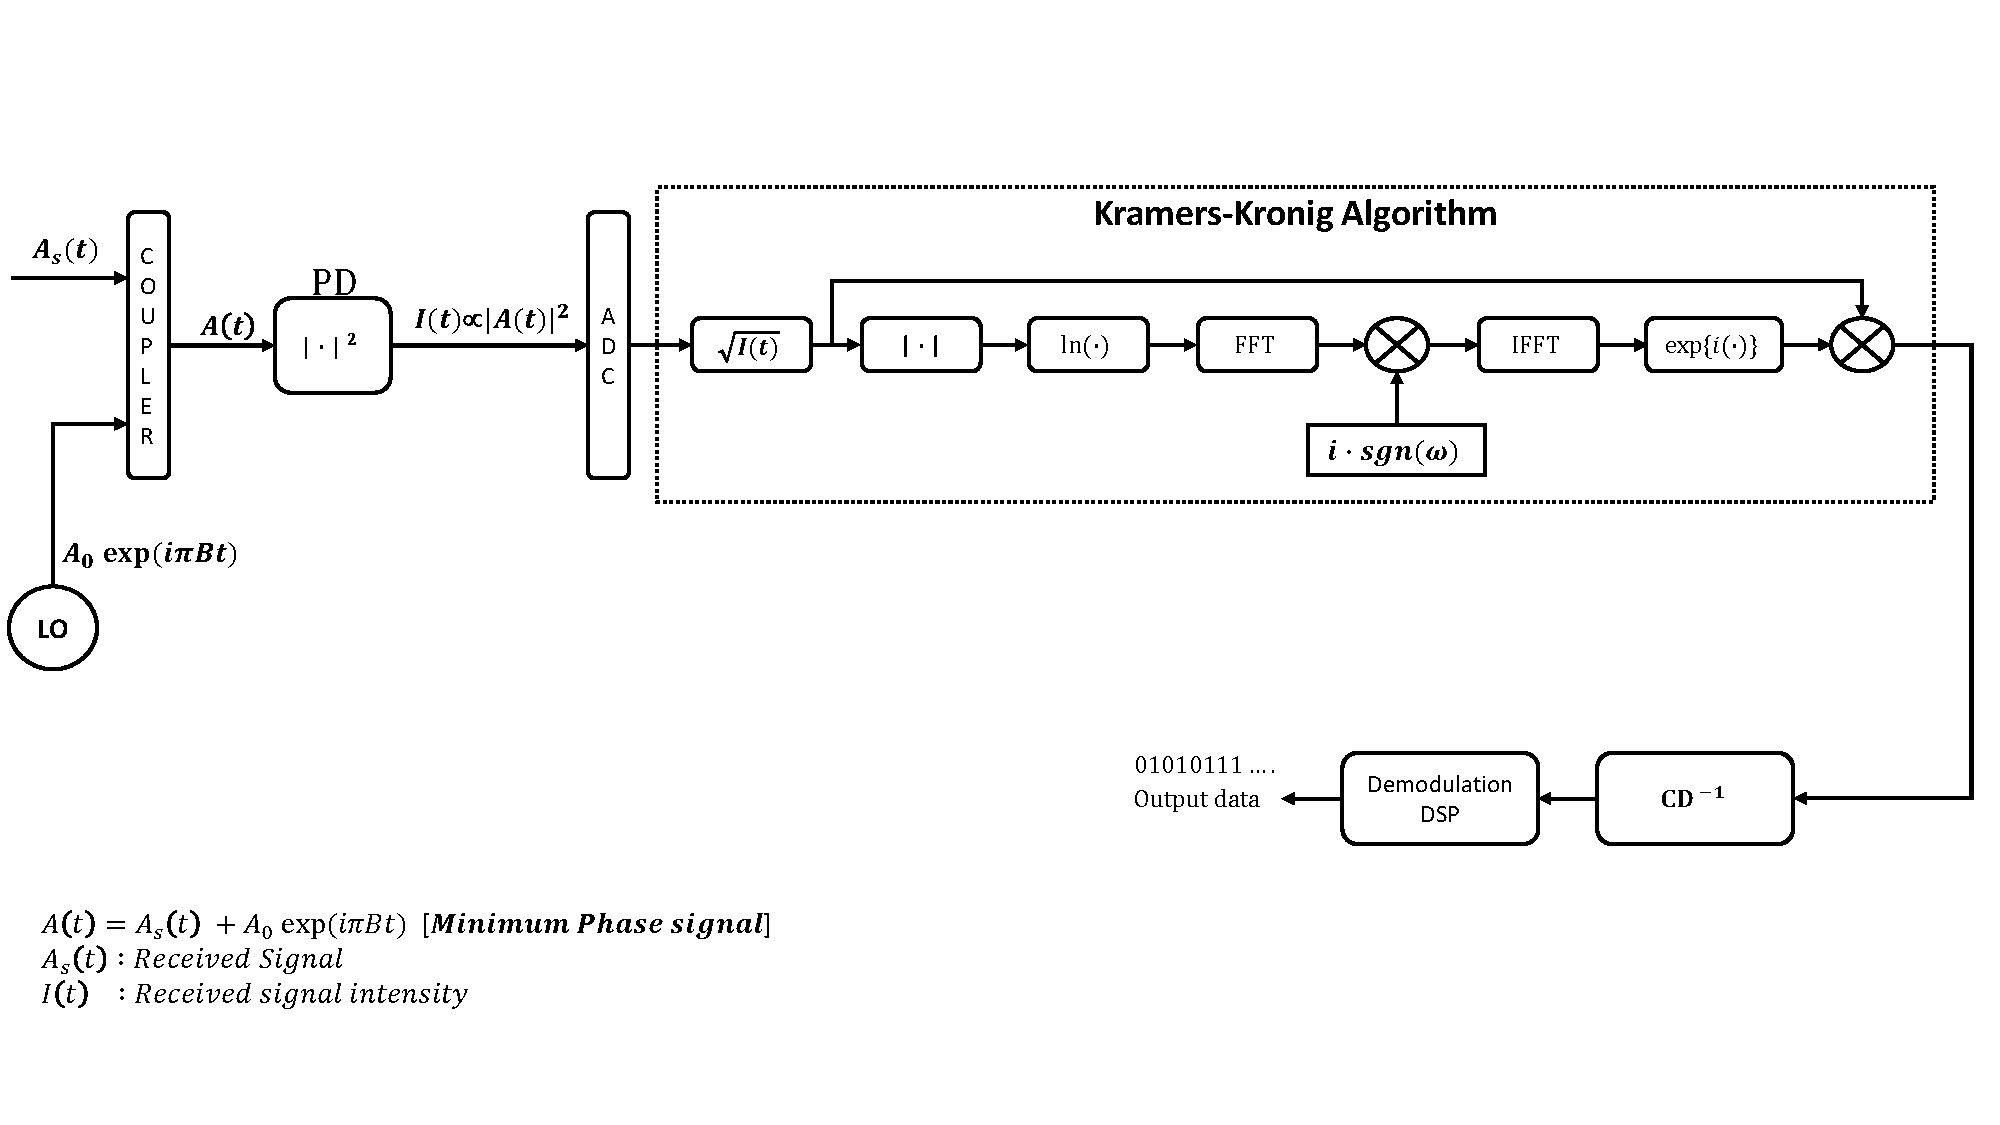
\includegraphics[width=1.0\textwidth, height=10cm]{./figures/Simulation_setup_Rx.pdf}
    \vspace{3mm}
    \caption{Receiver simulation setup}\label{}
\end{figure}
\end{itemize}

%--------------------------------------------------------------------------------------------------
%------------ SLIDE-------
\mysection{Experimental setup}\large
\begin{itemize}
  \item \textbf{Envisioned lab setup}
  \begin{figure}[hbt]
	\centering
	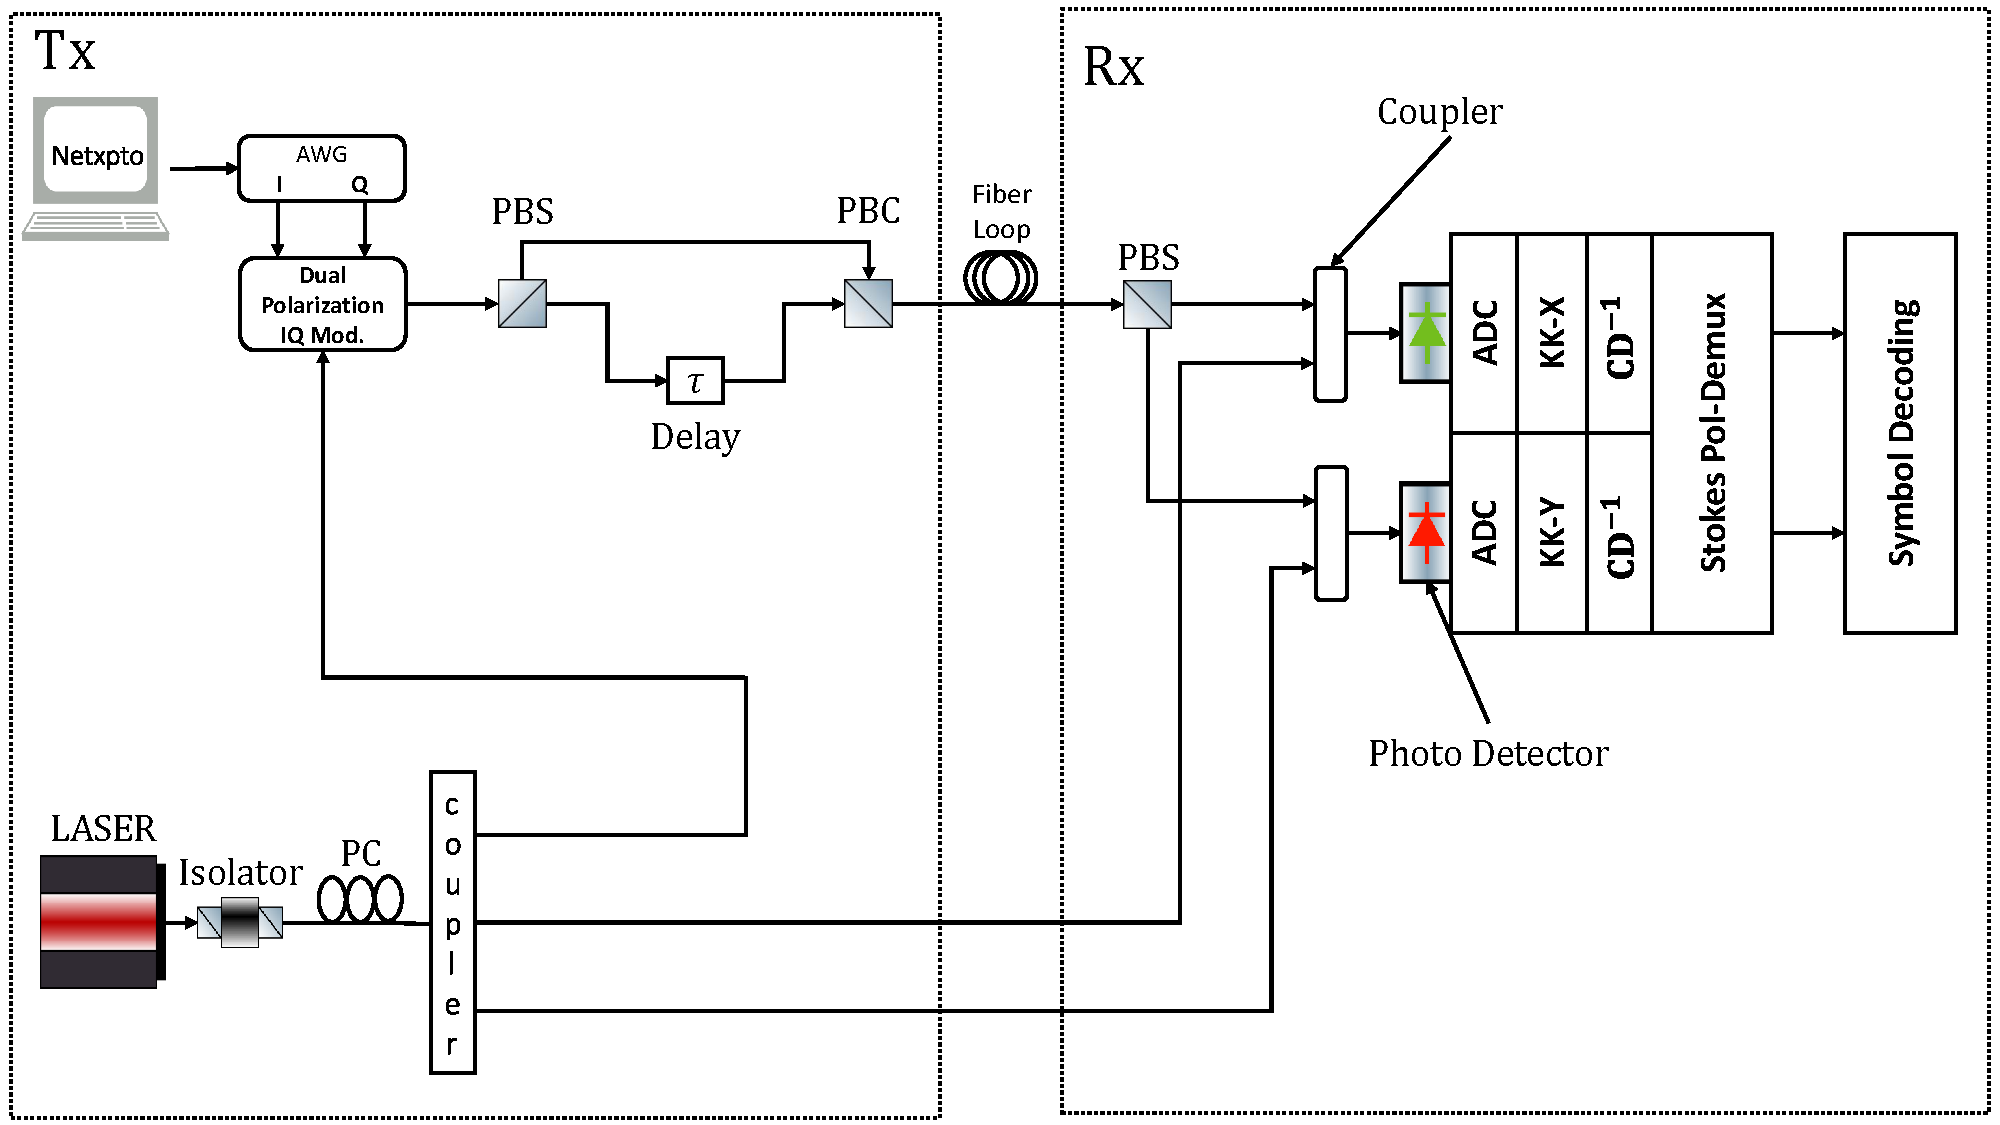
\includegraphics[width=1.0\textwidth, height=10cm]{./figures/Practical_setup_TxRx.pdf}
    \vspace{3mm}
    \caption{PDM Kramers-Kronig receiver experimental setup}\label{}
\end{figure}
\end{itemize}

%-------------------------------------------------------------------
%------------ SLIDE ------------------------------------------------
\mysection{} \sffamily
\vspace{-10mm}
\large\centerline{E-mail: marianaferreiraramos@ua.pt}


\end{document}
